\documentclass[pdftex,12pt,a4paper]{article}

\usepackage[slovak]{babel}
%\usepackage[IL2]{fontenc}
\usepackage[utf8]{inputenc}
\usepackage{fancyhdr}
\usepackage{mathtools}
\usepackage{hyperref}
\hypersetup{pdfborder={0 0 0}}
\usepackage[final]{pdfpages}
\usepackage{graphicx}
\usepackage{epstopdf}
\usepackage{subfigure}
\usepackage[top=3cm, bottom=3cm, right=2.5cm, left=2.5cm]{geometry}

\usepackage{listings}
\usepackage{color}
\usepackage{textcomp}
\definecolor{listinggray}{gray}{0.9}
\definecolor{lbcolor}{rgb}{0.95,0.95,0.95}
\lstset{
	backgroundcolor=\color{lbcolor},
	tabsize=4,
	rulecolor=,
	language=matlab,
        basicstyle=\scriptsize,
        upquote=true,
        aboveskip={0.3\baselineskip},
        columns=fixed,
        showstringspaces=false,
        extendedchars=true,
        breaklines=true,
        prebreak = \raisebox{0ex}[0ex][0ex]{\ensuremath{\hookleftarrow}},
        frame=single,
        showtabs=false,
        showspaces=false,
        showstringspaces=false,
        identifierstyle=\ttfamily,
        keywordstyle=\color[rgb]{0,0,1},
        commentstyle=\color[rgb]{0.133,0.545,0.133},
        stringstyle=\color[rgb]{0.627,0.126,0.941},
}

% matrix columns
\makeatletter
\renewcommand*\env@matrix[1][*\c@MaxMatrixCols c]{%
  \hskip -\arraycolsep
  \let\@ifnextchar\new@ifnextchar
  \array{#1}}
\makeatother

% norm command
\newcommand{\norm}[1]{\left|\left|#1\right|\right|}
% adj command
\newcommand{\adj}{\operatorname{adj}}
% rank command
\newcommand{\rank}{\operatorname{rank}}
% m command (matrix)
\newcommand{\m}[1]{\mathbf{#1}} 

\renewcommand{\labelitemi}{$\bullet$}


\def \nazovUlohy{Technická správa pre automat na jízdenky}
\def \skola{\textbf{ČVUT FEL - Kybernetika a Robotika}}
\def \tema{Úloha z APO (Architektúra počítačov)}
\def \author{\textbf{Michal Šustr} \\ \textbf{Matúš Cvengroš}}
\def \date{21. 4. 2012}

\fancyhead[L]{\skola \\ \nazovUlohy} 
\fancyhead[R]{\author}
\fancyfoot[C]{\thepage}
\renewcommand{\headrulewidth}{0.4pt}
\renewcommand{\footrulewidth}{0.4pt}
\renewcommand{\refname}{\section{Zoznam použitej literatúry}}

\hypersetup{
    bookmarks=true,         % show bookmarks bar?
    unicode=false,          % non-Latin characters in Acrobat’s bookmarks
    pdftoolbar=true,        % show Acrobat’s toolbar?
    pdfmenubar=true,        % show Acrobat’s menu?
    pdffitwindow=false,     % window fit to page when opened
    pdfstartview={FitH},    % fits the width of the page to the window
    pdftitle=\nazovUlohy,    % title
    pdfauthor=\author,     % author
    pdfsubject=\tema,   % subject of the document
    pdfnewwindow=true,      % links in new window
    colorlinks=true,       % false: boxed links; true: colored links
    linkcolor=blue,          % color of internal links
    citecolor=green,        % color of links to bibliography
    filecolor=magenta,      % color of file links
    urlcolor=blue           % color of external links
}


\begin{document}
\begin{center}
	\makebox[4cm][l]{
\includegraphics[width=3cm]{/home/michal/.latex/lev.png}}
	\parbox[s][4cm][s]{10cm}{\scshape \large
	České vysoké učení technické v Praze\\Fakulta elektrotechnická\\Katedra kybernetiky}
	\vskip 2cm {\Huge \bfseries \nazovUlohy}
	\vskip 1cm {\Large \tema}
\end{center}

\vfill

\begin{flushright}
	\author \\
	~\\
	\date
\end{flushright}


\newpage
\pagestyle{fancy}
Karta má 8 lediek, LCD displej s dvomi riadkami o 16 znakoch, a 14 tlačidiel na klávesnici.

O prácu s kartou sa starajú funkcie deklarované v súbore \texttt{device.h}. Nasleduje výpis dôležitých funkcií:
\begin{itemize}\itemsep5pt
	\item \texttt{void turn\_on(int device)} \\  zapne kartu s identifikátorom \texttt{device}, v našom prípade \texttt{0x1f321172}. Pre kartu používa globálnu premennú \texttt{mem}, preto sa dá naraz pracovať iba s jedinou kartou.
	\item \texttt{void turn\_off()} \\ vypne kartu
	\item \texttt{void start\_sound()} \\  spustí bzučák
	\item \texttt{void stop\_sound()} \\  zastaví bzučák
	\item \texttt{void read\_data(int addr)} \\  zo zadanej adresy prečíta dáta	
	\item \texttt{void write\_data(int addr, int data)} \\  na zadanú adresu zapíše dáta
	\item \texttt{void write\_led(int data)} \\  zápis 8-bitového čísla na LED-ky
	\item \texttt{void hide\_leds()} \\  zhasne všetky LED-ky
	\item \texttt{void show\_led\_parade()} \\  postupne zapne jednu LED-ku za druhou
	\item \texttt{void initialize\_lcd()} \\  pred zápisom na LCD je potrebné zavolať inicializáciu
	\item \texttt{void write\_lcd(int line, int position, char c)} \\  zapíše znak \texttt{c} na riadok \texttt{line} (začíname od 0) na pozíciu \texttt{position} \\  (tiež od 0)
	\item \texttt{void write\_lcd\_line(char *string, int line)} \\  zapíše dlhši reťazec od začiatku riadku pokiaľ sa zmestí (\texttt{line} je buď 0 alebo 1, čiže 1. alebo 2. riadok)
\newpage
	\item \texttt{int read\_keyboard()} \\ vráti index klávesy ktorá bola stlačená alebo -1 pre žiadnu klávesu. Tabuľka kláves: 
\begin{figure}[htb]
	\begin{center}
		\leavevmode
		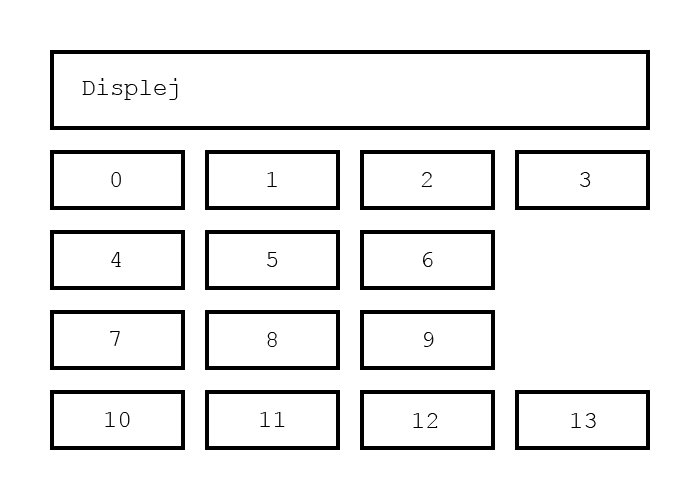
\includegraphics[width=0.6\textwidth]{klavesy.png}
	\end{center}
\end{figure}

\end{itemize}

Samotná implementácia automatu sa nachádza v súbore \texttt{main.c}. V nekonečnej smyčke program čaká na stlačenie kláves a vypisuje aký je aktuálny stav nákupu. Mince na zásobníku sa ukladajú do binárneho súboru uloženého v \texttt{/tmp/coins}, pričom tento súbor sa aktualizuje po každom nákupe.

Stlačením kontrolnej sekvencie \texttt{CTRL+C} v termináli sa prípravok bezpečne ukončí a vypne.
\end{document}